% arara: pdflatex: { synctex: yes, shell: yes }

% A primeira linha do ficheiro indica ao programa 'arara' como compilar
% o documento. Existem várias maneiras diferentes de compilar, mas esta
% primeira linha pode em geral ser ignorada.

% Este comando, o primeiro do documento, importa a classe a usar. Cada
% documento só pode ter uma classe.
\documentclass[portuguese]{ist-thesis}

% Entre 'documentclass' e 'begin{document}' encontra-se o 'preamble', ou
% a secção de código para importar packages e estabelecer configurações
% para o documento todo. A classe importa algumas packages básicas por
% defeito, mas aqui estão outras packages também úteis para uma tese.
% Qualquer package pode ser importada, que em geral não gera conflito.
% Recomendo consultar a documentação de cada package no site 'ctan.org'.

% Configurações para citações internacionais
\usepackage{csquotes}

% Gestão de bibliografia e citações
\usepackage{biblatex}
\addbibresource{main.bib}

% Introdução de texto de exemplo
\usepackage{lipsum}

% Estilo diferente de tabelas
\usepackage{booktabs}

% Glossários
\usepackage[abbreviations,symbols]{glossaries-extra}
\setabbreviationstyle{long-short}
\loadglsentries{glossary}

% Packages para esboçar gráficos e diagramas
\usepackage{tikz}
\usepackage{pgfplots}
\usetikzlibrary{positioning,arrows.meta}

% Alterar as pastas de onde importar imagens (/graphics/) e dados de
% vários tipos (/data/)
\graphicspath{{graphics/}}
\pgfplotsset{table/search path = {data}}

% Comando próprio da classe
% Define a imagem de capa pelo nome, com o tamanho entre parênteses
% retos (fracção da largura da página, neste caso metade)
\setcoverimage[0.5]{example-image-a}

% Fim do 'preamble' e início do documento escrito
\begin{document}

% Comando próprio da classe
% Cria a capa com base nos dados fornecidos no 'preamble' com comandos
% próprios
\makecover

% Ambiente próprio da classe
% Formata o texto no seu interior como dedicatória
\begin{dedication}
	\lipsum[1] % Introduz um parágrafo de 'lorem ipsum', ou texto exemplo
\end{dedication}

% Ambiente próprio da classe
% Formata o texto no seu interior como agradecimentos
\begin{acknowledgements}
	\lipsum[2] % Introduz um parágrafo de 'lorem ipsum', ou texto exemplo
\end{acknowledgements}

% Ambiente próprio da classe
% Formata o texto no seu interior como resumo, aceitando palavras-chave
% como um argumento extra
\begin{tabstract}{Resumo, Palavras-Chave, Resumo Analítico}
	Resumo e palavras-chave (em português e em inglês). O resumo analítico, também designado por resumo ou abstract, descreve o objectivo, o conteúdo do trabalho e as conclusões. Deve ser escrito em português e inglês, com um máximo de 250 palavras cada e acompanhado de 4 a 6 palavras-chave.
\end{tabstract}

% Ambiente próprio da classe
% Igual ao ambiente anterior mas para a língua oposta à principal
\begin{fabstract}{Abstract}
	The abstract describes the objective, the content of the project and the conclusions. It must be written in both portuguese and english, with a maximum of 250 words, accompanied by 4 to 6 keywords.
\end{fabstract}

% Índice
\tableofcontents

% Lista de figuras
\listoffigures

% Lista de tabelas
\listoftables

% Glossários
\printunsrtglossary[style = long, nogroupskip]
\printunsrtglossary[type = abbreviations, style = long, nogroupskip, title = {Lista de Acrónimos}]
\printunsrtglossary[type = symbols, nogroupskip, title = {Lista de Símbolos}]

% Comando próprio da classe
% Finaliza a parte inicial do documento, e começa o texto escrito
% propriamente dito. Utilizado pela classe para definir coisas como
% o tipo de numeração
\mainstart

\chapter{Introduction}



\section{Motivation}

Electronic badges are present in multiple fields. There are a vast number of possible applications. Some of them are:

\begin{itemize}
    \item \textbf{Corporate and business events} - Attendee identification, control the secure areas within events, networking and data exchange between badges 
    \item \textbf{Healthcare} - Patient identification in hospitals and clinics, monitoring and tracking healthcare workers and patients for safety and security
    \item \textbf{Tourism} - Keyless entry to hotel rooms or Airbnb accommodations, access to theme parks, concerts, and other entertainment events
    \item \textbf{Wharehousing} - Inventory management and order fulfillment
    \item \textbf{Fitness} - Monitoring and tracking athletes' performance and health, gamification of fitness activities to encourage physical activity
    \item \textbf{Entertainment and Gaming} - Collectible or interactive gaming badges at conventions and events, scavenger hunts and interactive experiences at theme parks
    \item \textbf{Marketing and Brand Promotion} - Collecting data on consumer behavior and preferences at trade shows and events, and personalized marketing and advertising based on that data
\end{itemize}

\section{Requirements/who is this for}

This electronic badge is aimed at new students entering IST, and it will have the following features:

\begin{itemize}
    \item \textbf{Student Identification} - Name, Student ID, IST email, phone number and course. This data can be configured and altered by the user and also shared between users through IR
    \item \textbf{A treasure hunt game}, where students will explore the campus, and enter a code every time they encounter a new location
    \item \textbf{Games} - to be played on a small display and on a serial monitor when connected to a computer through USB
\end{itemize}

There are two extra, but fundamental requirements: the whole board shouldn't cost more than 10€, and it should be as energy efficient as possible, lasting at least around two days without being recharged. 

It's important to keep a balance between the power consumption: the time the board lasts, the functionality, and the cost. The goal isn't to make a board that can run the most high-end games, if it is expensive and the battery runs out too fast. The opposite is also applicable, a board that lasts a lot of time, but doesn't give the user a good experience doesn't meet the requirements. So, the objective is to find a medium point, where some compromises are made in order to keep an overall balance and all requirements are met.  

\part{Introdução Teórica}

\chapter{Primeiro Capítulo}

\section{Similar projects}

It is crucial to recognize and analyze some of the current badges that have served as the foundation for this study as we delve into the world of electronic badges. These earlier badges serve as illustrations of comparable field implementations, offering insightful comparisons and standards against which our badge can be evaluated. 

The first notable example is a badge built for Hacker Hotel, an annual technology and hacker conference that takes place in the Netherlands. For the 2023 edition, they designed a puzzle game in the board intended to entertain the visitors, taking them around the venue where the event took place, and to find clues to an eventual solution. The badge has a row of push buttons for users to input the binary codes of each clue. It uses an RP2040 microcontroller is powered by a CR2032 coin cell. 

\begin{figure}[ht]
	\centering
	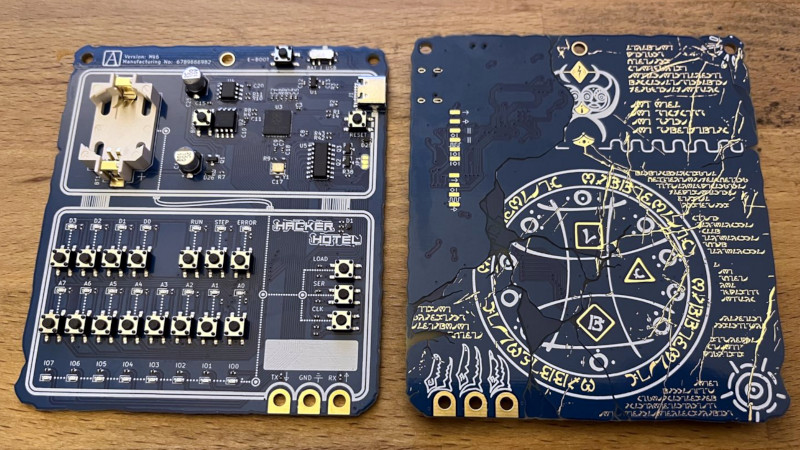
\includegraphics[width = 0.8\linewidth]{images/hacker_hotel.jpg}
	\caption{Hacker Hotel 2023 badge.}
	\label{fig:hacker_hotel}
\end{figure}

One drawback of this badge is that it only has utilty for the Hacker Hotel event, not anything beyond. 

\section{Possible Solutions}

As for the input interface, one option is to put four directional arrow buttons, and an additional pair of buttons denoted as "A" and "B," serving as functional equivalents to "OK" and "Cancel. With this type of button interface, the student is allowed to do everything asked in the requirements - see and change personal information, play the treasure hunt game, and the normal games. 

\section{Energy saving}



\section{SPI Protocol}

The Serial Peripheral Interface (SPI) works by using 4 lines:

\begin{itemize}
  \item \textbf{MOSI (Master Output/Slave Input)} - Line that carries data from the Master to the Slave
  \item \textbf{MISO (Master Input/Slave Output)} - Line that carries data from the Slave to the Master
  \item \textbf{SCLK (Serial Clock)} - Clock line generated by the master device to synchronize data transfer
  \item \textbf{SS/CS - (Slave Select/Chip Select)} - Line used by the master to select the specific slave device it wants to communicate with.
\end{itemize}

\begin{figure}[ht]
	\centering
	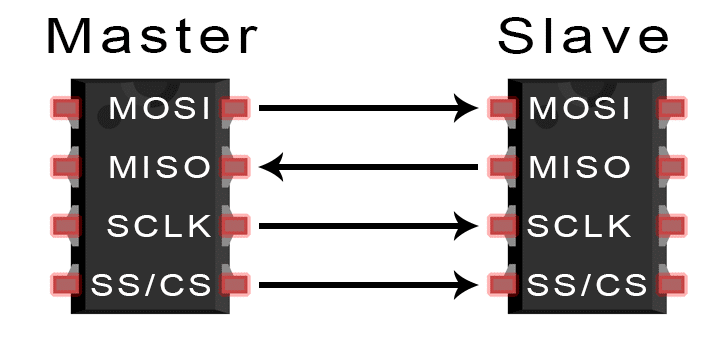
\includegraphics[width = 0.5\linewidth]{images/protocolos/SPI_master_slave.png}
	\caption{SPI.}
	\label{fig:spi}
\end{figure}

The communication starts with the master assigning a slave to send data to. It does that by setting the SS/CS line to low. When it is  in idle mode, not transmitting, the line is set to high. Then the master sends the clock signal to synchronize the output of data bits from the master to the sampling of bits by the slave (meaning this is a synchronous communication protocol). In each clock cycle, one bit of data is transmitted, so the speed of the communication is determined by the clock frequency. The data sent from the master to the slave is transmitted trough the MOSI line, and it is usually sent with the most significant bit first. In the MISO line, the data is sent from the slave to the master, and usually with the least significant bit first. After the data transfer, the master changes the state of the SS/CS line, indicating the end of the communication with a particular slave. 

\section{I2C Protocol}

Unlike the SPI protocol, the I2C (Inter-Integrated Circuit) protocol works using only 2 lines:

\begin{itemize}
  \item \textbf{SDA (Serial Data)} - Line that carries data between the slave and the master
  \item \textbf{SCL (Serial Clock)} - Line that provides the clock signal that synchronizes data transfer.
\end{itemize}

The devices both transmit and receive data in the same line, the SDA. The data is transmitted in messages, that are composed of different frames (groups of bits). The message is composed of:

\begin{itemize}
  \item \textbf{One start bit}, where the SDA line switches from 1 to 0
  \item \textbf{An address frame}, 7 or 10 bits that identify the slave with which the communication is being done
  \item \textbf{An ACK/NACK bit}, sent by the slave that the master wants to communicate to, to confirm if the slave received the address frame, by changing the SDA line from high to low.
  \item \textbf{The data frame}, which is always 8 bits, and sent starting with the most significant bit. It's also followed by an ACK/NACK bit. The message can have multiple data frames.
  \item \textbf{A stop bit} to end the message, sent by the master by switching the SDA line from 0 to 1.
\end{itemize}

\begin{figure}[ht]
	\centering
	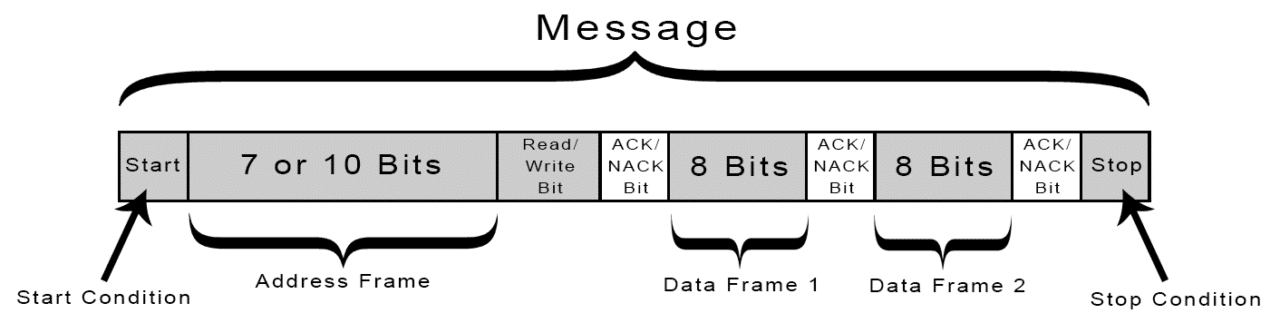
\includegraphics[width = 0.8\linewidth]{images/protocolos/i2c_message.png}
	\caption{I2C.}
	\label{fig:i2c}
\end{figure}

\section{UART}

The UART (Universal Asynchronous Receiver/Transmitter) is not a communication protocol, unlike SPI and I2C, it is a physical circuit in a microcontroller whose purpose is to transmit and receive data. 

UART uses 2 wires, connected to 2 pins:

\begin{itemize}
    \item \textbf{Tx} - To transmit data
    \item \textbf{Rx} - To receive data
\end{itemize}

\begin{figure}[ht]
	\centering
	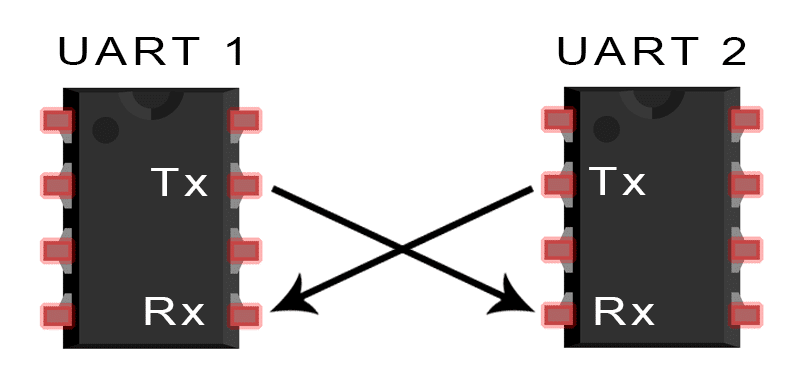
\includegraphics[width = 0.8\linewidth]{images/protocolos/uart.png}
	\caption{UART.}
	\label{fig:uart}
\end{figure}

Data flows from the Tx pin to the Rx pin, and it doesn't use a clock signal, so it is an asynchronous communication method. To indicate the beginning and the end of the message, start and stop bits are added to the data frame. In order to be synchronized, the devices that are communicating configure the correspondent frequency at which the data is transmitted and received, which is called the baud rate, and must be the same in both devices. 

The UART data packet is composed of:

\begin{itemize}
    \item \textbf{Start bit} - The UART device pulls the transmission line from high to low, to indicate the start of the transmission
    \item \textbf{Data frame} - 5 to 8 bits sent from the least to the most significant bit, which contain the data that is being transmitted.
    \item \textbf{Parity bit} -  The bits can be altered by electromagnetic radiation, different baud rates, long transmissions, so the parity bit allows the receiving device to know if the data has been corrupted during the transmission. It works by counting the number of 1s in the data frame. If that number is even, the parity bit must be zero; if the number is odd, the parity bit must be 1. The receiver then confirms if the parity bit and the number of 1 bits match
    \item \textbf{Stop bit} - The UART transmitting device pulls the line from high to low for at least two bits
\end{itemize}

\section{SPI vs I2C vs UART}

Both protocols have their advantages and disadvantages, which are important to consider. I2C is simpler in terms of wiring because it only uses 2 lines, unlike SPI which uses 4. However, this works in favor of the SPI protocol, because the MOSI and MISO lines enable the devices to receive and transmit data at the same time. 
Regarding slave addressing, the SPI protocol has a specific line for it, which makes it easier than sending the slave address in each message (even though in SPI, if multiple slaves are used, the master needs to have a different SS/CS pin for each one). SPI only supports one master, while I2C can have multiple master. 
Another difference between the two protocols is that SPI doesn't need start and stop bits, so it can stream data continuously. On the other hand, I2C has an ACK bit that confirms if the message was received correctly.



Energy saving is a big focus point in this project, so it's also crucial to analyze the difference in power consumption between each communication protocol.

Explicar tmb aqui a velocidade, por causa do open colector?

\section{Display Choice}

The two main goals are to keep the power consumption as low as possible, as well as the price of the board. Thus, it's important to choose the right display for this application, because it will be the most energy costly and the most expensive component. Various displays with various types of technologies were considered and compared (LCD, OLED and ePaper). 

\subsection{LCD}
LCD (Liquid Crystal Display) 

\subsection{OLED}
OLED (Organic Light Emitting Diode)
One advantage that the OLED has over LCD displays is that it is thinner

\subsection{ePaper}
Another option to consider for the display is an ePaper display. 
The way they work is by utilizing a thin film of micro-capsules backed by an electrode panel. Each capsule contains millions of ink-particles that are electrically charged and suspended on clear fluid. By applying negative and positive charges to the electrodes the ink different ink particles get attracted or repelled, thus creating an image. This explains why these types of displays don't need power to maintain what is displayed on the screen. Only when the image changes does it require power. 

\begin{table}[ht]
	\centering                 
	\caption{Algumas expressões e variáveis. Nas tabelas, a legenda vem em cima.}
	\begin{tabular}{| c | c | c |}
            \hline
		- & - & - \\
		\hline
		- & - & - \\
		\hline
		- & - & - \\
		\hline
		- & - & - \\
		\hline
	\end{tabular}
	\label{tab:displays}
\end{table}

\section{Primeira Secção}

Esta referência liga à equação \eqref{eq:equation1}.

\begin{gather}\label{eq:equation1}
	\mathbb{P}\left(\frac{X_1 + \cdots + X_n}{\sqrt{n}} \leq y\right) \rightarrow \mathrm{R}(y) = \int_{-\infty}^{y} \frac{e^{-t^2/2}}{\sqrt{2\pi}}dt \qquad \mathrm{as} \quad n \rightarrow \infty
\end{gather}

\begin{figure}[ht]
	\centering
	\includegraphics[width = 0.5\linewidth]{example-image}
	\caption{Imagem de exemplo.}
	\label{fig:image1}
\end{figure}

\lipsum[1] % Introduz um parágrafo de 'lorem ipsum', ou texto exemplo

\begin{table}[ht]
	\centering
	\caption{Algumas expressões e variáveis. Nas tabelas, a legenda vem em cima.}
	\begin{tabular}{c c c}\toprule
		\textbf{Função}		& \textbf{Valor de $\mathbf{x}$}	& \textbf{Valor de $\mathbf{y}$}\\
		\midrule
		$y = 4x$			& $67$								& $268$							\\
		$y = x^2$			& $13$								& $169$							\\
		$y = e^x$			& $9.5$								& $33.115$						\\
		\bottomrule
	\end{tabular}
	\label{tab:tab1}
\end{table}

\lipsum[11] % Introduz um parágrafo de 'lorem ipsum', ou texto exemplo

\begin{figure}[ht]
	\centering
	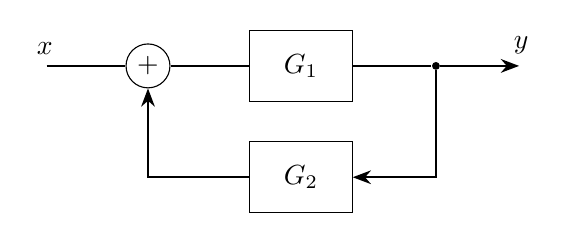
\begin{tikzpicture}
		\tikzstyle{mainblock} = [rectangle, draw, align = center, minimum height = 9mm, minimum width = 13mm];
		\tikzstyle{sum} = [circle, draw, align = center, inner sep = 2pt];
		\tikzstyle{mainpath} = [draw, thick, -{Stealth[]}];
		\node (start) at (0,0) [inner sep = 0mm, label = {90:$x$}] {};
		\node (sum1) [sum, right=of start] {$+$};
		\node (g1) [mainblock, right=of sum1] {$G_1$};
		\node (ex1) [circle, fill, inner sep = 1pt, right=of g1] {};
		\node (end) [right=of ex1, inner sep = 0mm, label = {90:$y$}] {};
		\node (g2) [mainblock, below=5mm of g1] {$G_2$};
		\path [mainpath] (start) -- (sum1) -- (g1) -- (ex1) -- (end);
		\path (ex1) -- (ex1 |- g2) [mainpath] --  (g2);
		\path (g2) -- (g2 -| sum1) [mainpath] -- (sum1);
	\end{tikzpicture}
	\caption{Exemplo de um diagrama feito em \LaTeX{}.}
	\label{fig:diag1}
\end{figure}

\lipsum[13] % Introduz um parágrafo de 'lorem ipsum', ou texto exemplo

\begin{figure}[h]
	\centering
	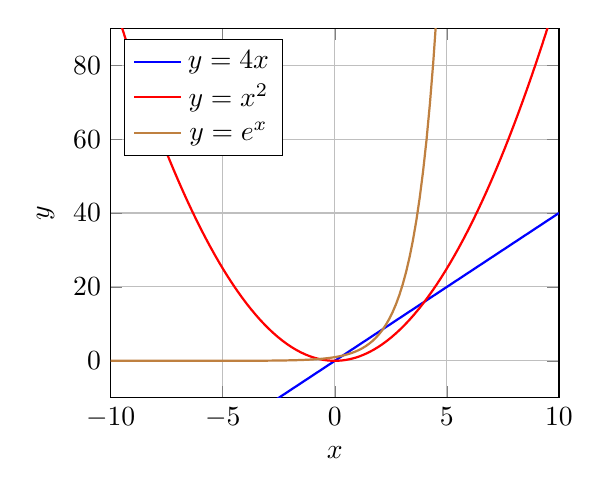
\begin{tikzpicture}
		\begin{axis}
				[width = 0.6\linewidth,
				samples = 100,
				grid = both,
				xmin = -10, xmax = 10,
				ymin = -10, ymax = 90,
				xlabel = {$x$},
				ylabel = {$y$},
				legend pos = north west,]
			\addplot [mark = none, color = blue, thick, domain = -10:10] {4*x};
			\addplot [mark = none, color = red, thick, domain = -10:10] {x^2};
			\addplot [mark = none, color = brown, thick, domain = -10:5] {e^x};
			\legend{$y = 4x$,$y = x^2$,$y = e^x$};
		\end{axis}
	\end{tikzpicture}
	\caption{Exemplo de um gráfico em \LaTeX{}.}
	\label{fig:graph1}
\end{figure}

\part{Implementação e Resultados}

\lipsum[15] % Introduz um parágrafo de 'lorem ipsum', ou texto exemplo

\begin{figure}
	\centering
	\begin{tikzpicture}
		\begin{axis}
				[width = 0.9\linewidth,
				height = 0.6\linewidth,
				xmin = 5,
				grid = both,
				xlabel = {Tempo ($x$)},
				ylabel = {Amplitude},
				legend pos = north east,]
			\addplot [red] table [col sep = comma, x index = 0, y index = 1, mark = none] {data_example.csv};
			\legend{Exemplo};
		\end{axis}
	\end{tikzpicture}
	\caption[Exemplo de um gráfico de dados em \LaTeX{}.]{Exemplo de um gráfico de dados em \LaTeX{}. Os dados foram obtidos de um ficheiro \texttt{.csv} externo.}
	\label{fig:graph2}
\end{figure}

\lipsum % Introduz um parágrafo de 'lorem ipsum', ou texto exemplo

% Citações vazias. Permite à bibliografia incluir as referências sem
% citações no texto.
\nocite{latex-companion, fontcatalogue, latexwiki, ctan, texsx}

\part{Bibliografia e Apêndices}

% Introduz a bibliografia. A opção 'heading = bibintoc' introduz a
% bibliografia no índice.
\printbibliography[heading = bibintoc]

% Começar o apêndice. A estrutura dos capítulos é a mesma que no documento
% principal.
\appendix

\chapter{Primeiro Anexo}

\lipsum

\chapter{Segundo Anexo}

\lipsum

\makespine

\end{document}
